\section{Einführung}

\begin{frame}
	\frametitle{Induction Logic Programming -- ILP}

	\begin{block}{Was ist ILP}
		\begin{itemize}
			\item Die Schnittstelle zwischen Machine Learning und logischer Programmierung
			\item {Idee: Formalisierung der \textit{Umgebung}
				\begin{itemize}
					\item Basis: Background-Knowledge, positive und negative Beispiele
					\item Darstellung in Form von Klauseln
					\item Generierung neuen Wissens durch das finden von Hypothesen die positive
					Klauseln erfüllen, negative jedoch nicht.
				\end{itemize}
			}
		\end{itemize}
	\end{block}
	Wieso induktiv?
	$\Rightarrow$ Lösen von Problemen vom spezifischen zum generellen
\end{frame}

\subsection{First order logic}
\begin{frame}
	\frametitle{First order logic -- FOL}
	\begin{block}{}
	In \textbf{FOL} besteht die Welt aus
	% TODO: Begriffe nochmal genauer anschauen: Insbesondere Atome
	\begin{itemize}
		\item Objekten  Personen, Dingen)
		\item Prädikaten $(>, <)$
		\item Funktionen $(+, -)$
	\end{itemize}
	\end{block}


	Terme beschreiben Objekte in der Welt:\\
	Konstanten ($2$, Chuck Norris), Variablen (x,y, a, \ldots) und
	Funktionen von Termen sind Terme.

	\textit{Ground term}: Ein Term ohne Variablen.

	\begin{block}{}
		Atome/Literale sind kleinstmögliche Ausdrücke, die wahr/falsch sind
		\begin{itemize}
			\item $predicate(Term_1, \ldots, Term_n)$\\ 
				Beispiel: is\_human(Pinoccio)
			\item $Term_1 = Term_2$ (Gleicheitsrelation)
		\end{itemize}
	\end{block}

\end{frame}

\begin{frame}
	\frametitle{Art der Logik -- Beispiel}

	\begin{block}{Welt}
		$\text{Konstante} = \{\text{Zero}\}$\\
		$\text{Funktion} =\{Succ/1, Plus/2 \}$\\
		$\text{Prädikate} =\{even/1, is\_greater/2 \}$
	\end{block}

	Interpretation $\mathcal{I}$ besitzt eine Grundmenge $\mathcal{M}$
	und bildet Konstanten und Funktionen auf Elemente der Grundmenge ab.

	Prädikate werden auf Wahrheitswerte abgebildet

	\begin{block}{Interpretation}
			$\mathcal{M} = \mathbb{N}_0$\\
			$\mathcal{I}(Zero) = 0$\\
			$\mathcal{I}(Plus(Succ(Zero), Succ(Zero))) = 2$\\
			$\mathcal{I}(even(Suc(Suc(Zero)))) = True$
	\end{block}
	
\end{frame}

\begin{frame}
	\frametitle{First order logic und ILP}
	Horn Clauses: Klausel mit maximal einem negativen Literal.

	\begin{align*}
		\neg C_1 \vee \neg C_2 \vee \ldots \vee \neg C_n  \vee C_{n+1} \Leftrightarrow\\
		C_1 \wedge C_2 \wedge \ldots \wedge C_n  \rightarrow C_{n+1}
	\end{align*}

	ILP verwendet zumeist \textit{definite program clauses}(genau ein negatives Literal) vom Typ:

	\begin{align*}
		\underbrace{T}_{\text{head}} \Leftarrow \underbrace{L_1, \ldots, L_m}_{\text{body}}
	\end{align*}
	wobei $T, L_1, \ldots, L_m$ Literale sind, wobei $T$ immer positiv ist.

	Beispiel:
	\begin{align*}
		daughter(X,Y) \Leftarrow female(X), mother(Y, X)
	\end{align*}
\end{frame}


\begin{frame}
\frametitle{Hypothesen, Beispiele etc}
	\emph{Gegeben:} Background-Knowledge $(B)$, Menge von positiven $(E^+)$ und negativen $(E^-)$ Beispielen\\
	\emph{Ziel:} Finden einer Hypothese $(\mathcal{H})$ die alle positiven und kein negatives Beispiele erfüllt
\begin{figure}[H]
	\centering
	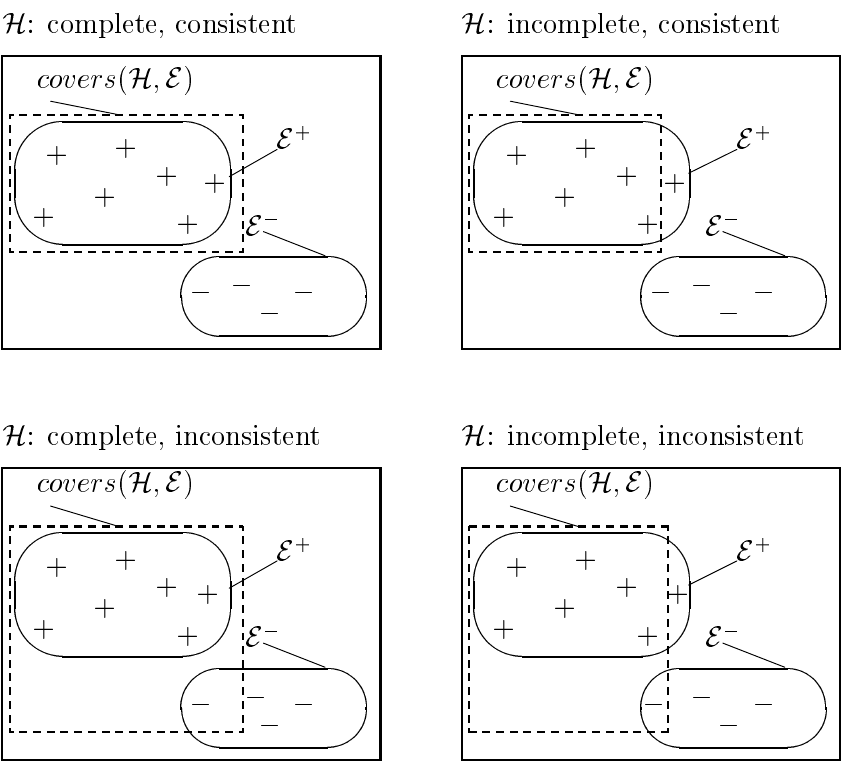
\includegraphics[width=0.5\textwidth]{hypothesis}
\end{figure}
\end{frame}
